%%%%%%%%%%%%%%%%%%%%%%%%%%%%%%%%%%%%%%%%%%%%%%%%%%%%%%%%%%%%%%%%%%%%
%% I, the copyright holder of this work, release this work into the
%% public domain. This applies worldwide. In some countries this may
%% not be legally possible; if so: I grant anyone the right to use
%% this work for any purpose, without any conditions, unless such
%% conditions are required by law.
%%%%%%%%%%%%%%%%%%%%%%%%%%%%%%%%%%%%%%%%%%%%%%%%%%%%%%%%%%%%%%%%%%%%

% This theme was based on fibeamer theme 
% If you found any bugs please contact @karlosos
% This repository is hosted on github https://github.com/karlosos/zut-fibeamer/

\documentclass[c]{beamer}
\usetheme[faculty=wi]{fibeamer}
\usepackage[utf8]{inputenc}
\usepackage[
  main=portuguese,
  english
]{babel}

\title{Impacto das modulações do {IEEE 802.15.4g} na qualidade de comunicação em ambiente de \textit{Smart Building}}
\subtitle{Discente: Felipe Ferreira Bezerra da Silva}
\author{Orientador: Prof. Ruan Delgado Gomes, D.Sc.}

\usepackage{ragged2e}  % `\justifying` text
\usepackage{booktabs}  % Tables
\usepackage{tabularx}
\usepackage{tikz}      % Diagrams
\usetikzlibrary{calc, shapes, backgrounds}
\usepackage{amsmath, amssymb}
\usepackage{url}       % `\url`s
\usepackage{listings}  % Code listings
\usepackage{graphicx}
\usepackage{multirow}
\usepackage{makecell}


\frenchspacing
\begin{document}
\frame[c]{\maketitle}

\AtBeginSection[]{% Print an outline at the beginning of sections
  \begin{frame}<beamer>
    \frametitle{Seção \thesection}
    \tableofcontents[currentsection]
  \end{frame}}

\begin{darkframes}

  \section{Introdução}
  \begin{frame}{Introdução}
    \framesubtitle{IoT}
    \begin{figure}[ht]
      \centering
      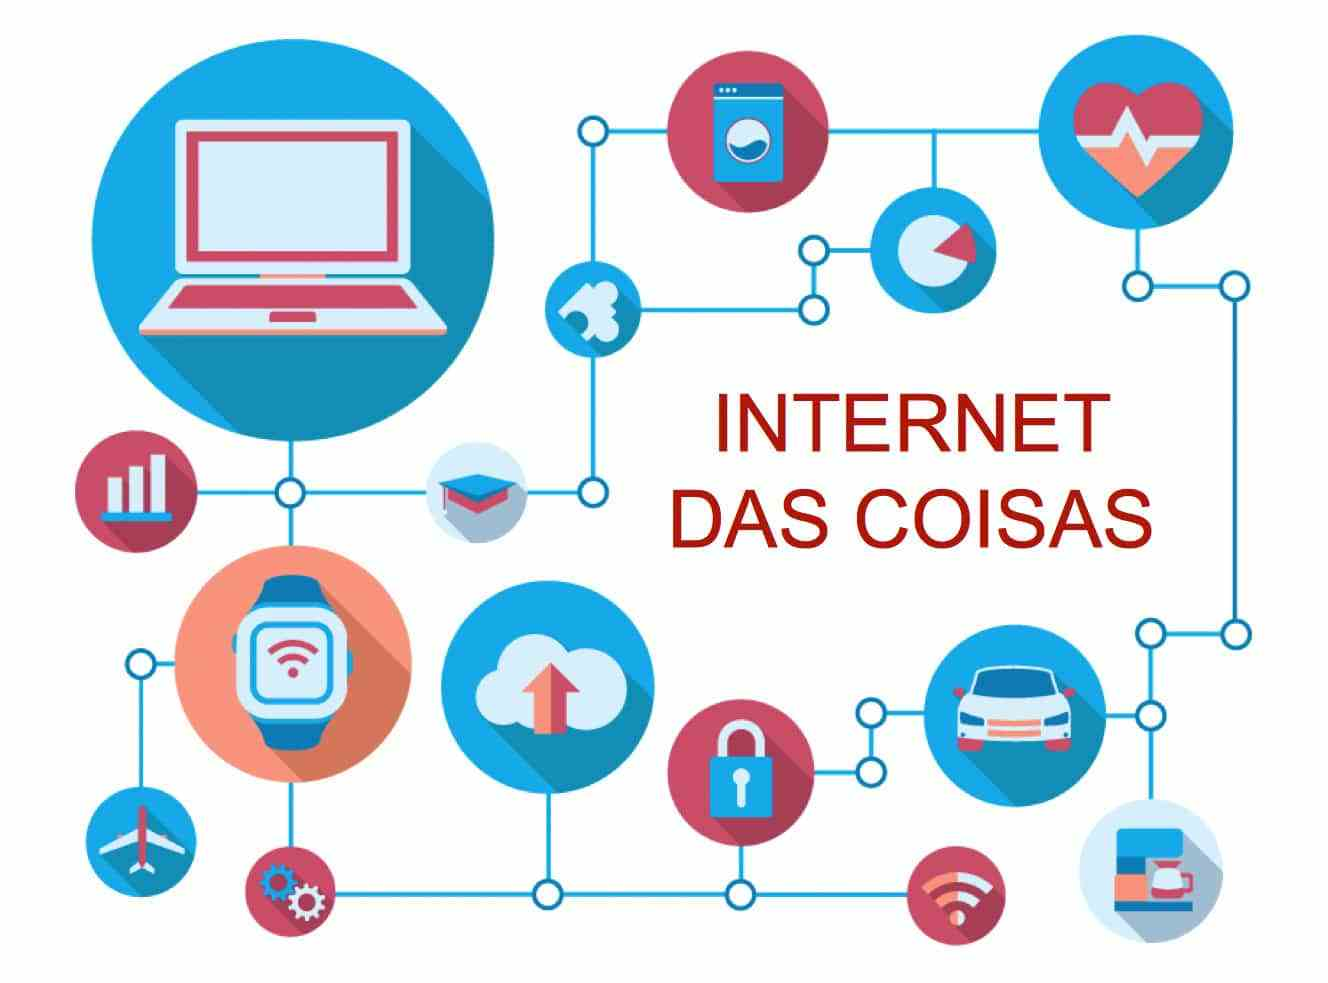
\includegraphics[width=.7\textwidth]{resources/intro_iot.jpg}\\
      \footnotesize{Disponível em  \url{http://sentrybrasil.com.br/cursos/internet-das-coisas-vai-revolucionar-o-mercado/}}
    \end{figure}
  \end{frame}

  \begin{frame}{Introdução}
    \framesubtitle{Aplicação - Smart Campus}
    \begin{figure}[ht]
      \centering
      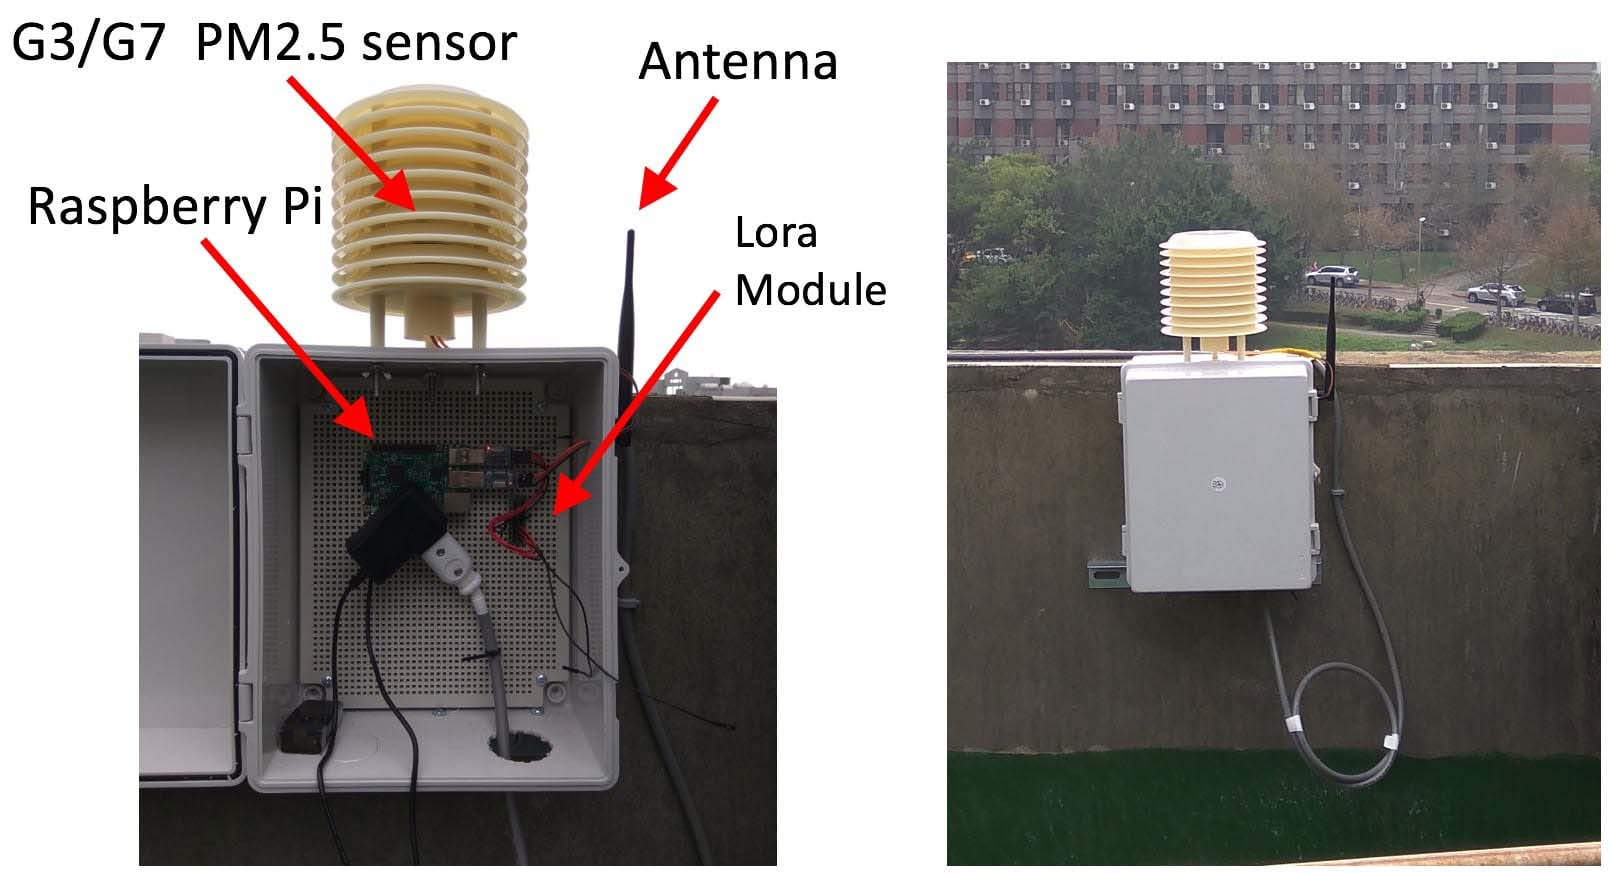
\includegraphics[width=.9\textwidth]{resources/smart-campus-example.png}\\
      \footnotesize{Retirado do artigo disponível em \url{https://ieeexplore.ieee.org/abstract/document/8288154}}
    \end{figure}
  \end{frame}

  \begin{frame}{Introdução}
    \framesubtitle{Aplicação - Smart Campus}
    \begin{figure}[ht]
      \centering
      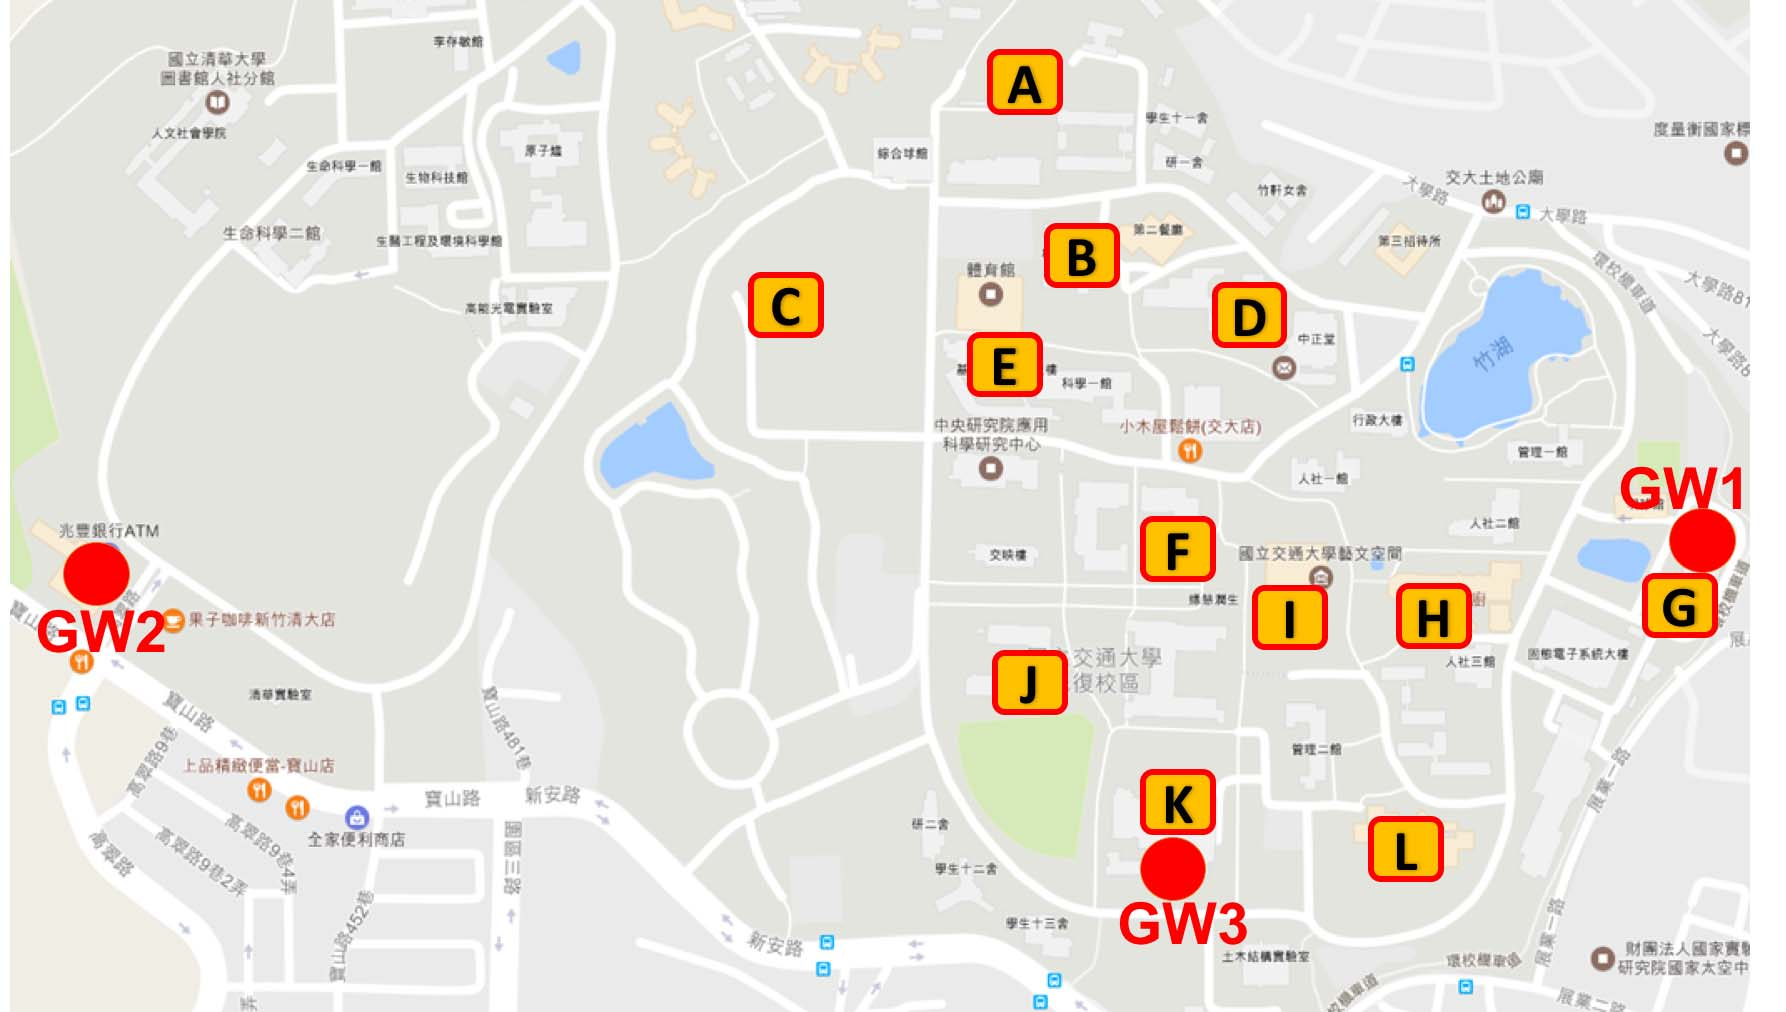
\includegraphics[width=.9\textwidth]{resources/smart-campus-locations.png}\\
      \footnotesize{Retirado do artigo disponível em \url{https://ieeexplore.ieee.org/abstract/document/8288154}}
    \end{figure}
  \end{frame}

  \begin{frame}{Introdução}
    \framesubtitle{Redes de Sensores Sem Fio}
    \begin{figure}[ht]
      \centering
      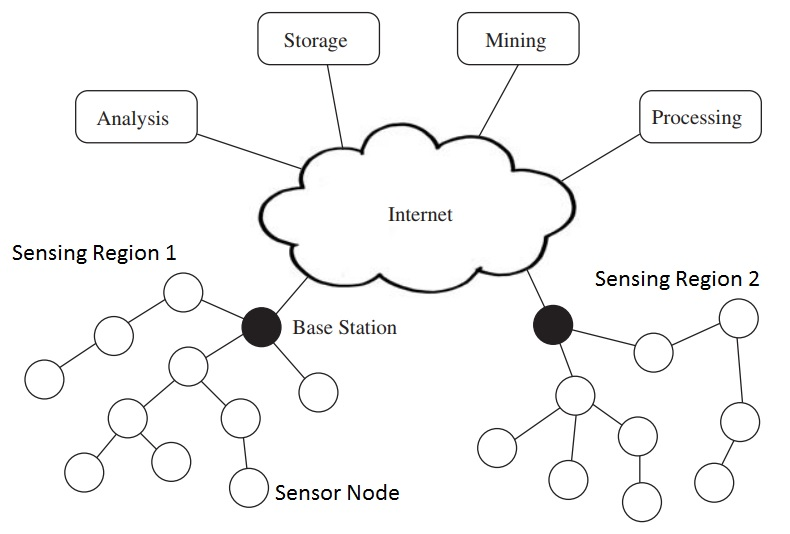
\includegraphics[width=.8\textwidth]{resources/Wireless-Sensor-Networks-WSN.jpg}\\
      \footnotesize{Disponível em  \url{https://getelectronicandmobilenews.blogspot.com/2019/03/basics-of-wireless-sensor-networks-wsn.html}}
    \end{figure}
  \end{frame}


  \begin{frame}{Introdução}
    \framesubtitle{Propagação por Multiplos Caminhos}
    \begin{figure}[ht]
      \centering
      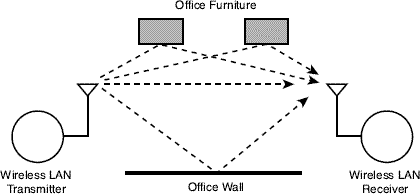
\includegraphics[width=\textwidth]{resources/multipath.png}\\
      \footnotesize{Disponível em  \url{https://sourcedaddy.com/networking/multipath-propagation.html}}
    \end{figure}
  \end{frame}

  \begin{frame}{Introdução}
    \framesubtitle{Interferência}
    \begin{itemize}
      \item \alert{Interferência Externa}             \\ Ocorre quando transmissores externos utilizam a mesma faixa de frequência
      \item \alert{Interferência Co-canal}            \\ Ocorre em sistemas com múltiplos usuários que utilizam o mesmo canal
      \item \alert{Interferência de Canal Adjacente}  \\ Ocorre quando uma transmissão é realizada muito proxima de um receptor que está recebendo transmissões de um outro transmissor
    \end{itemize}
  \end{frame}

  \begin{frame}{Introdução}
    \framesubtitle{Padrões e Tecnologias de Redes Sem Fio}
    \begin{figure}[ht]
      \centering
      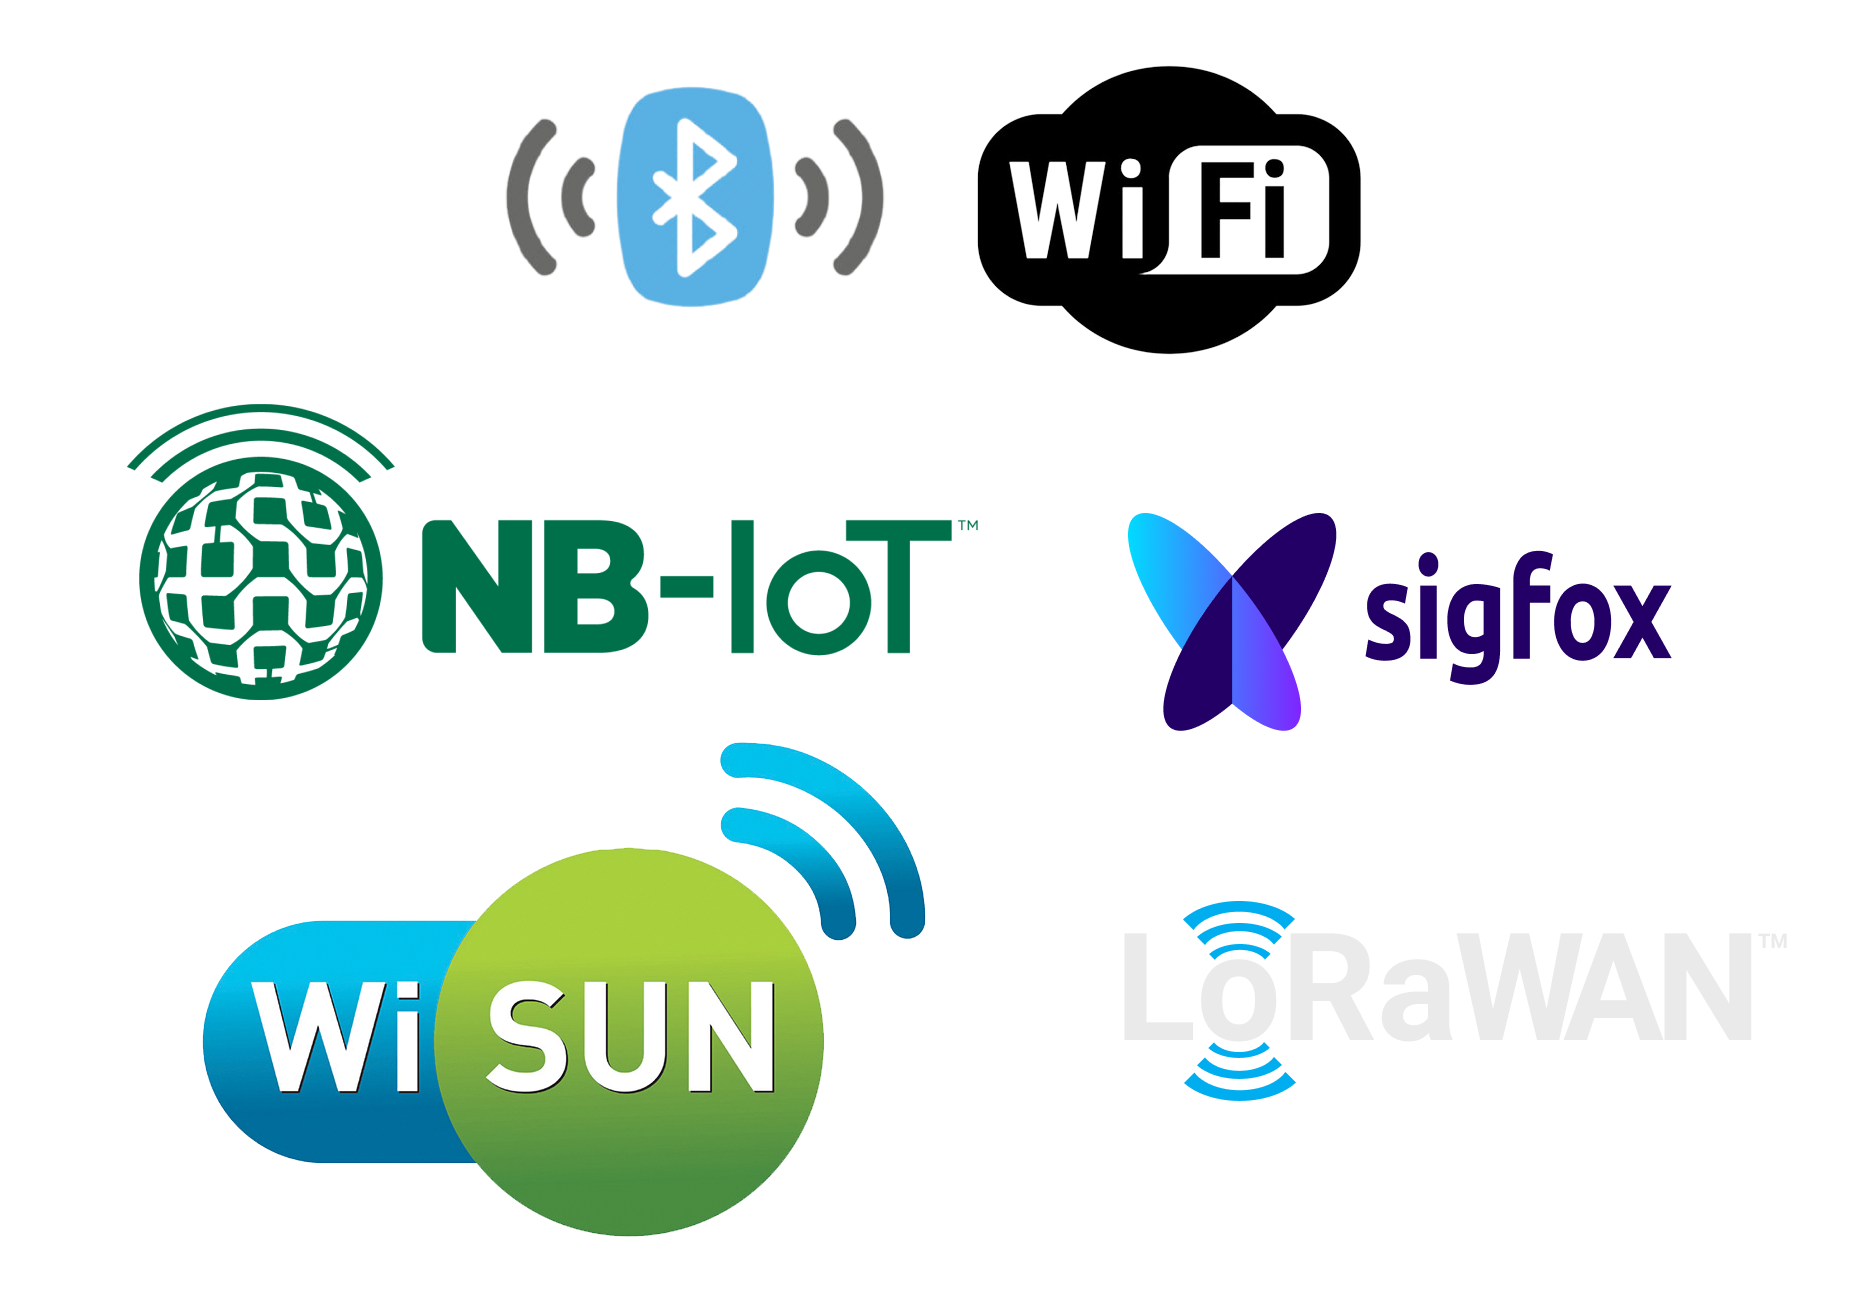
\includegraphics[width=0.8\textwidth]{resources/tecnologias-sem-fio.png}\\
      \footnotesize{Montagem criada pelo autor a partir das logos originais}
    \end{figure}
  \end{frame}

  \begin{frame}{Introdução}
    \framesubtitle{Justificativa e Relevância do Trabalho}
    \begin{figure}[ht]
      \centering
      Artigo \emph{A dataset to evaluate ieee 802.15.4g sun for dependable low-power wireless communications in industrial scenarios}
      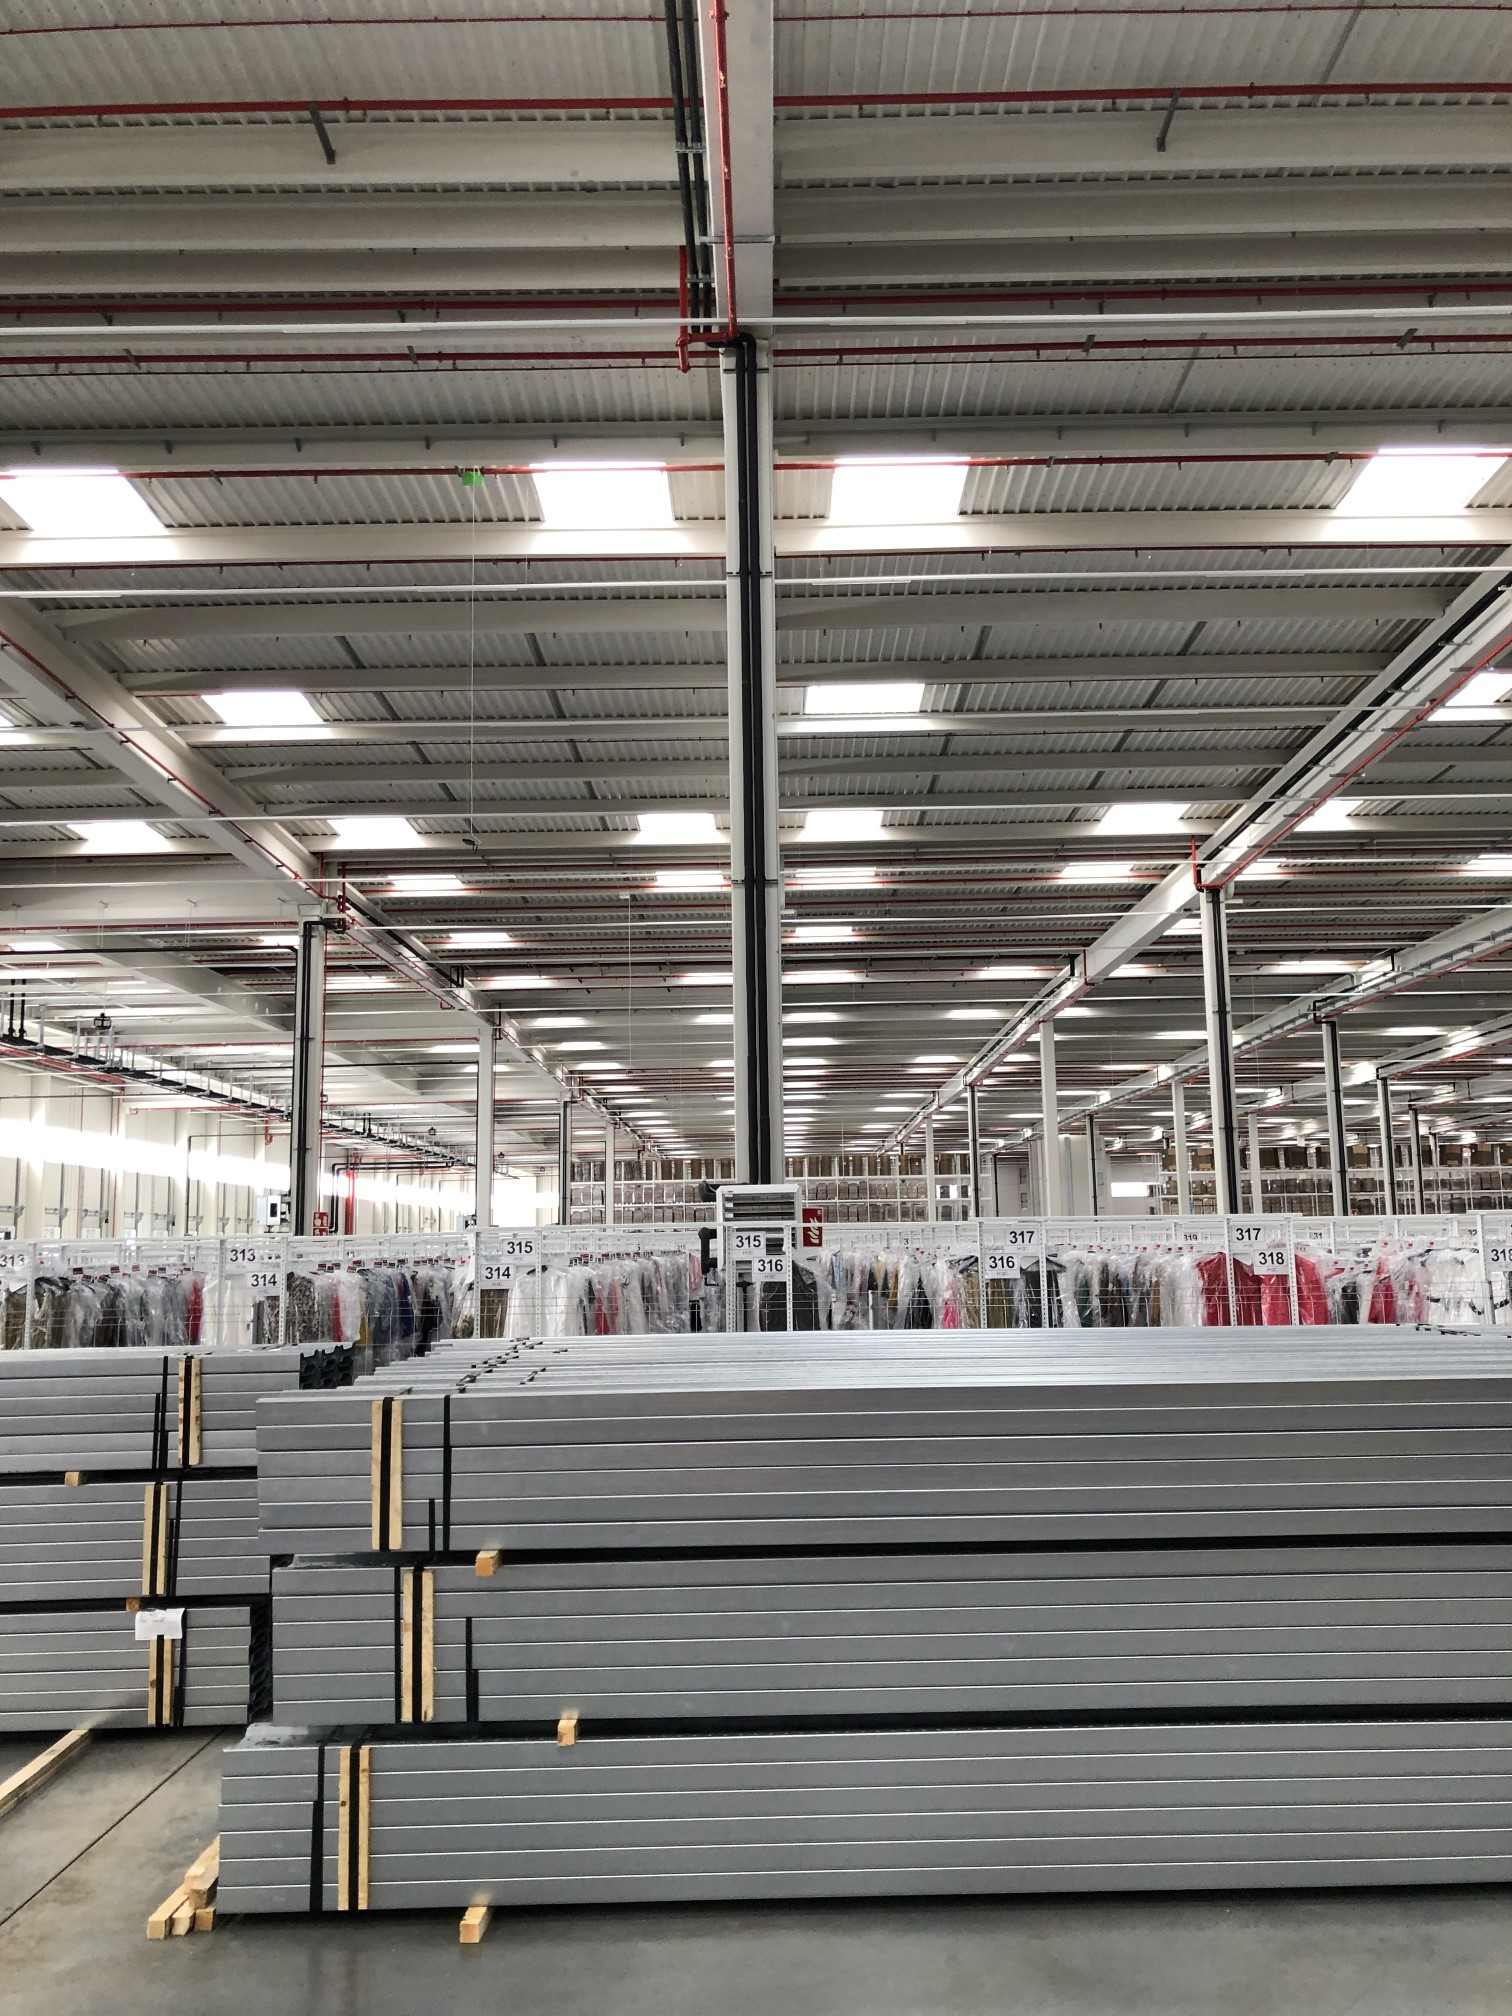
\includegraphics[width=0.3\textwidth]{resources/smart-industrie-example.png}
      \includegraphics[width=0.3\textwidth]{resources/smart-industrie-example2.png}
      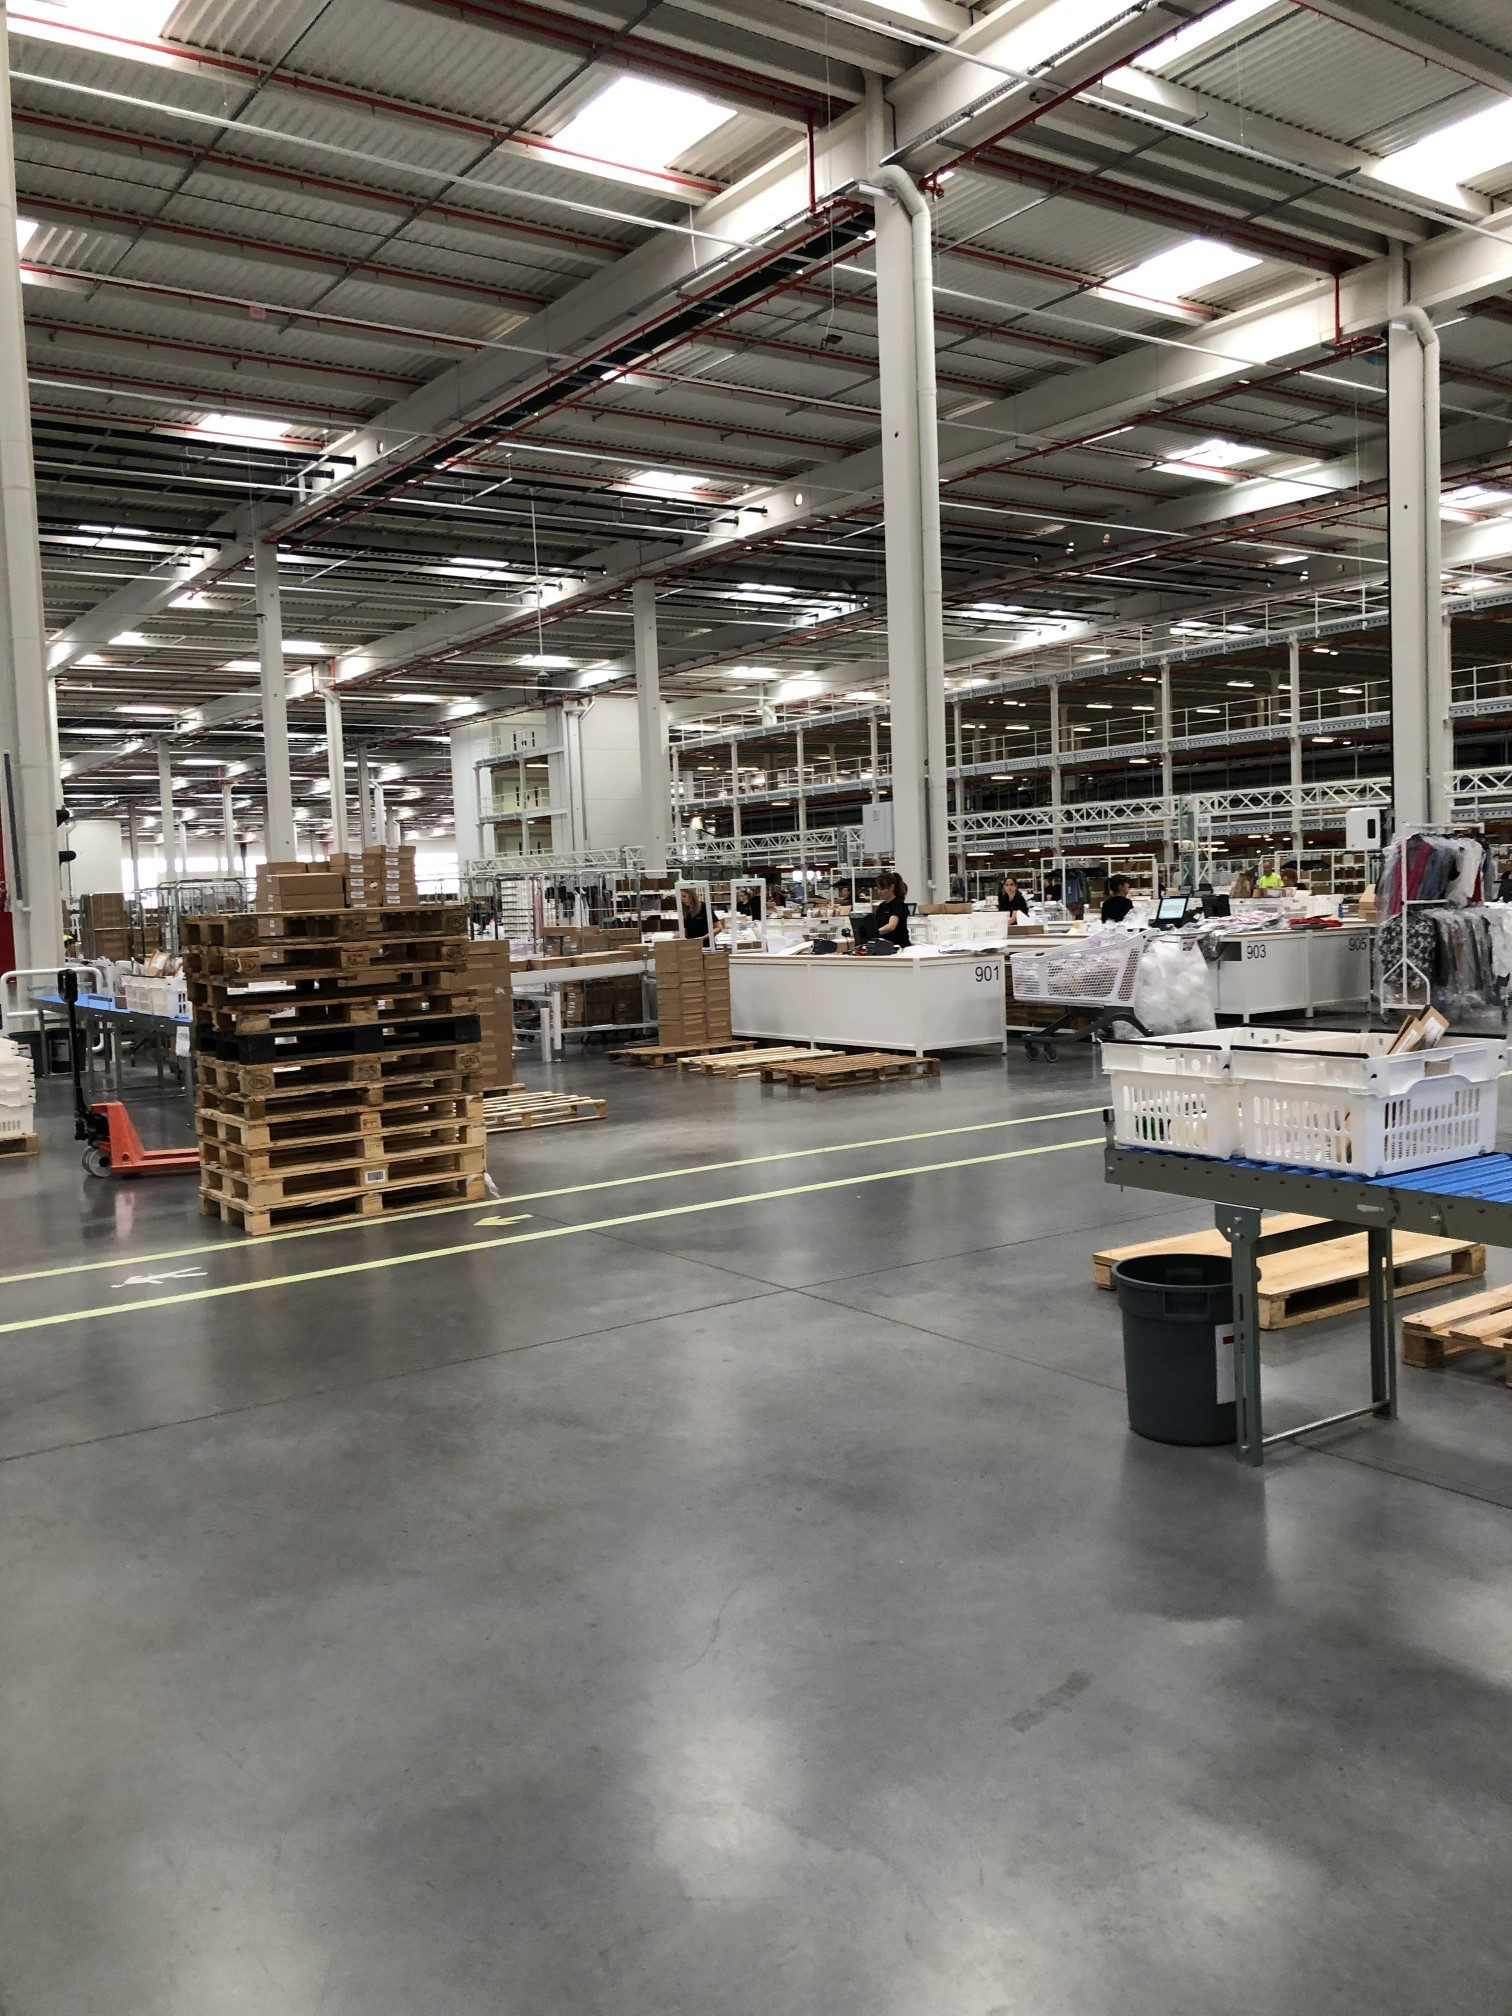
\includegraphics[width=0.3\textwidth]{resources/smart-industrie-example3.png}\\
      \footnotesize{Retirado do artigo disponível em \url{https://www.mdpi.com/2306-5729/5/3/64}}
    \end{figure}
  \end{frame}

  \begin{frame}{Introdução}
    \framesubtitle{Justificativa e Relevância do Trabalho}
    Coletar os dados de uma RSSF e analisar o desempenho as modulações \alert{SUN-FSK}, \alert{SUN-OQPSK} e \alert{SUN-OFDM}, definidas no padrão \alert{IEEE 802.15.4g SUN} no ambiente Smart Building

    \vskip .5cm

    \begin{block}{Desafios do cenário}
      \begin{itemize}
        \item Propagação por múltiplos caminhos
        \item Falta de linha de visada
      \end{itemize}
    \end{block}
  \end{frame}

  \section{IEEE 802.15.4g SUN}
  \begin{frame}{Modulações do IEEE 802.15.4g SUN}
    \framesubtitle{SUN-FSK}
    \begin{figure}
      \centering
      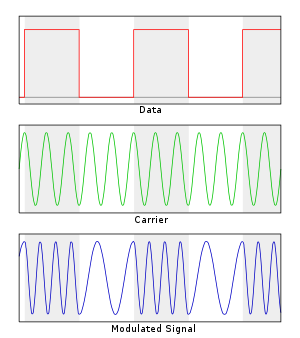
\includegraphics[width=.5\textwidth]{resources/Fsk.png}\\
      \footnotesize{Disponível em \url{https://en.wikipedia.org/wiki/Frequency-shift_keying}}
    \end{figure}
  \end{frame}

  \begin{frame}{Modulações do IEEE 802.15.4g SUN}
    \framesubtitle{SUN-FSK}
    \begin{exampleblock}{\begin{itemize}
          \item Eficiência energética
          \item Compatibilidade com sistemas legados
        \end{itemize}}
    \end{exampleblock}

    \begin{block}{Paramêtros}
      \begin{itemize}
        \item {Faixas de Frequência} - \char`~ 915 ou \char`~ 2400 MHz
        \item {Índice de Modulação} - 1,0 ou 0,5
        \item {Largura de banda do Canal} - 200 ou 400 kHz
        \item {Taxa de Transmissão} - {50}, {150} ou {200} k\emph{bits}/s
      \end{itemize}
    \end{block}
  \end{frame}

  \begin{frame}{Modulações do IEEE 802.15.4g SUN}
    \framesubtitle{SUN-OQPSK}
    \begin{figure}
      \centering
      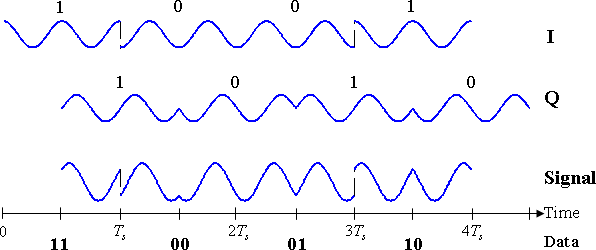
\includegraphics[width=\textwidth]{resources/OQPSK_timing_diagram.png}\\
      \footnotesize{Disponível em \url{https://en.wikipedia.org/wiki/Phase-shift_keying}}
    \end{figure}
  \end{frame}

  \begin{frame}{Modulações do IEEE 802.15.4g SUN}
    \framesubtitle{SUN-OQPSK}
    \begin{exampleblock}{
        \begin{itemize}
          \item Extendida do padrão IEEE 802.15.4
                \begin{itemize}
                  \item Novas \alert{faixas de frequência}
                  \item Diferentes \alert{fatores de espalhamento}
                \end{itemize}
          \item Suporta \alert{taxas de transmissão} de \alert{6,25} a até \alert{500} k\emph{bits}/s
        \end{itemize}}
    \end{exampleblock}
  \end{frame}

  \begin{frame}{Modulações do IEEE 802.15.4g SUN}
    \framesubtitle{SUN-OFDM}
    \begin{figure}
      \centering
      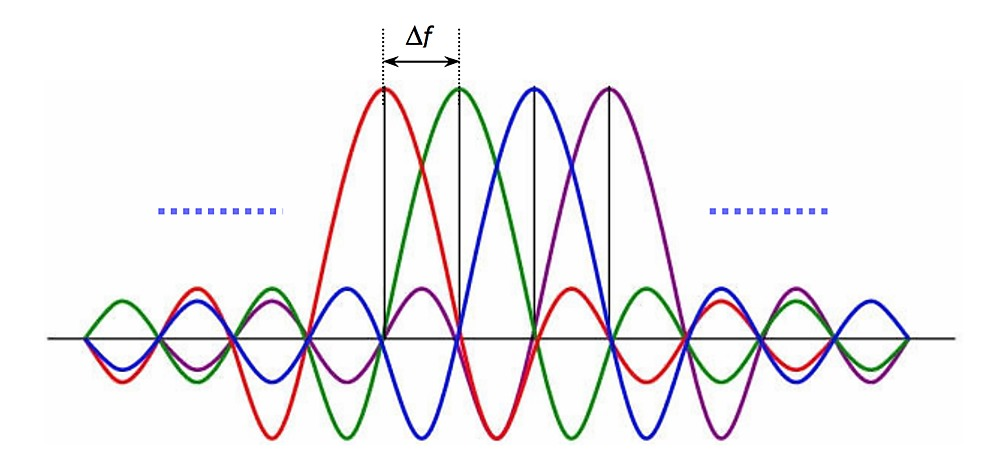
\includegraphics[width=\textwidth]{resources/ofdm.jpg}\\
      \footnotesize{Disponível em \url{https://figshare.com/articles/figure/ofdm-subcarriers/3470288/1}}
    \end{figure}
  \end{frame}

  \begin{frame}{Modulações do IEEE 802.15.4g SUN}
    \framesubtitle{SUN-OFDM}
    \begin{exampleblock}{
        \begin{itemize}
          \item Utiliza diferentes esquemas de modulação e codificação - BPSK, QPSK e 16-QAM
          \item Esquemas de repetição
          \item Largura de banda do canal - 200 e 1200 MHz
          \item Taxa de transmissão - 50 até 800 k\emph{bits}/s
        \end{itemize}}
    \end{exampleblock}
  \end{frame}

  \section{Experimento}
  \begin{frame}{Experimento}
    \framesubtitle{Visão Geral}
    \begin{figure}
      \centering
      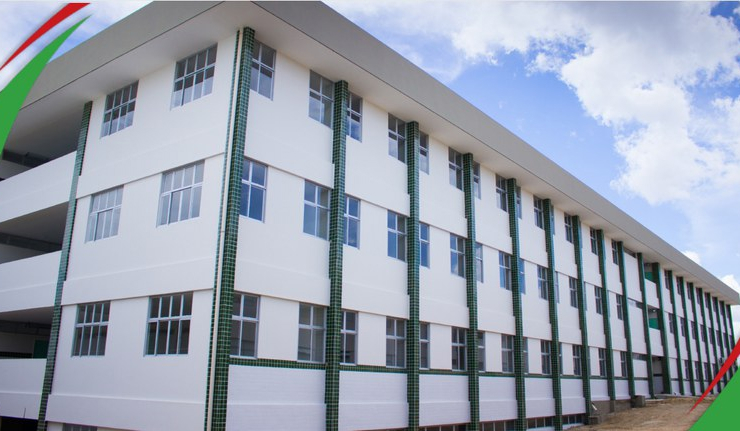
\includegraphics[width=0.53\textwidth]{resources/Subtract.jpg}
      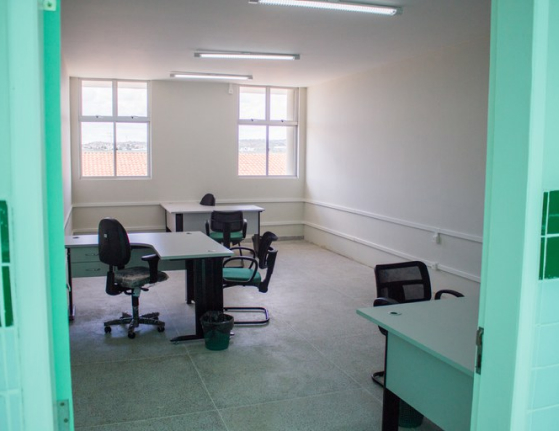
\includegraphics[width=0.4\textwidth]{resources/ifpb_sala.jpg}\\
      \footnotesize{Disponível em \url{https://www.ifpb.edu.br/noticias/2018/01/copy_of_ifpb-entrega-obra-inedita-na-rede-federal}}
    \end{figure}
  \end{frame}

  \begin{frame}{Experimento}
    \framesubtitle{Visão Geral}
    \begin{figure}
      \centering
      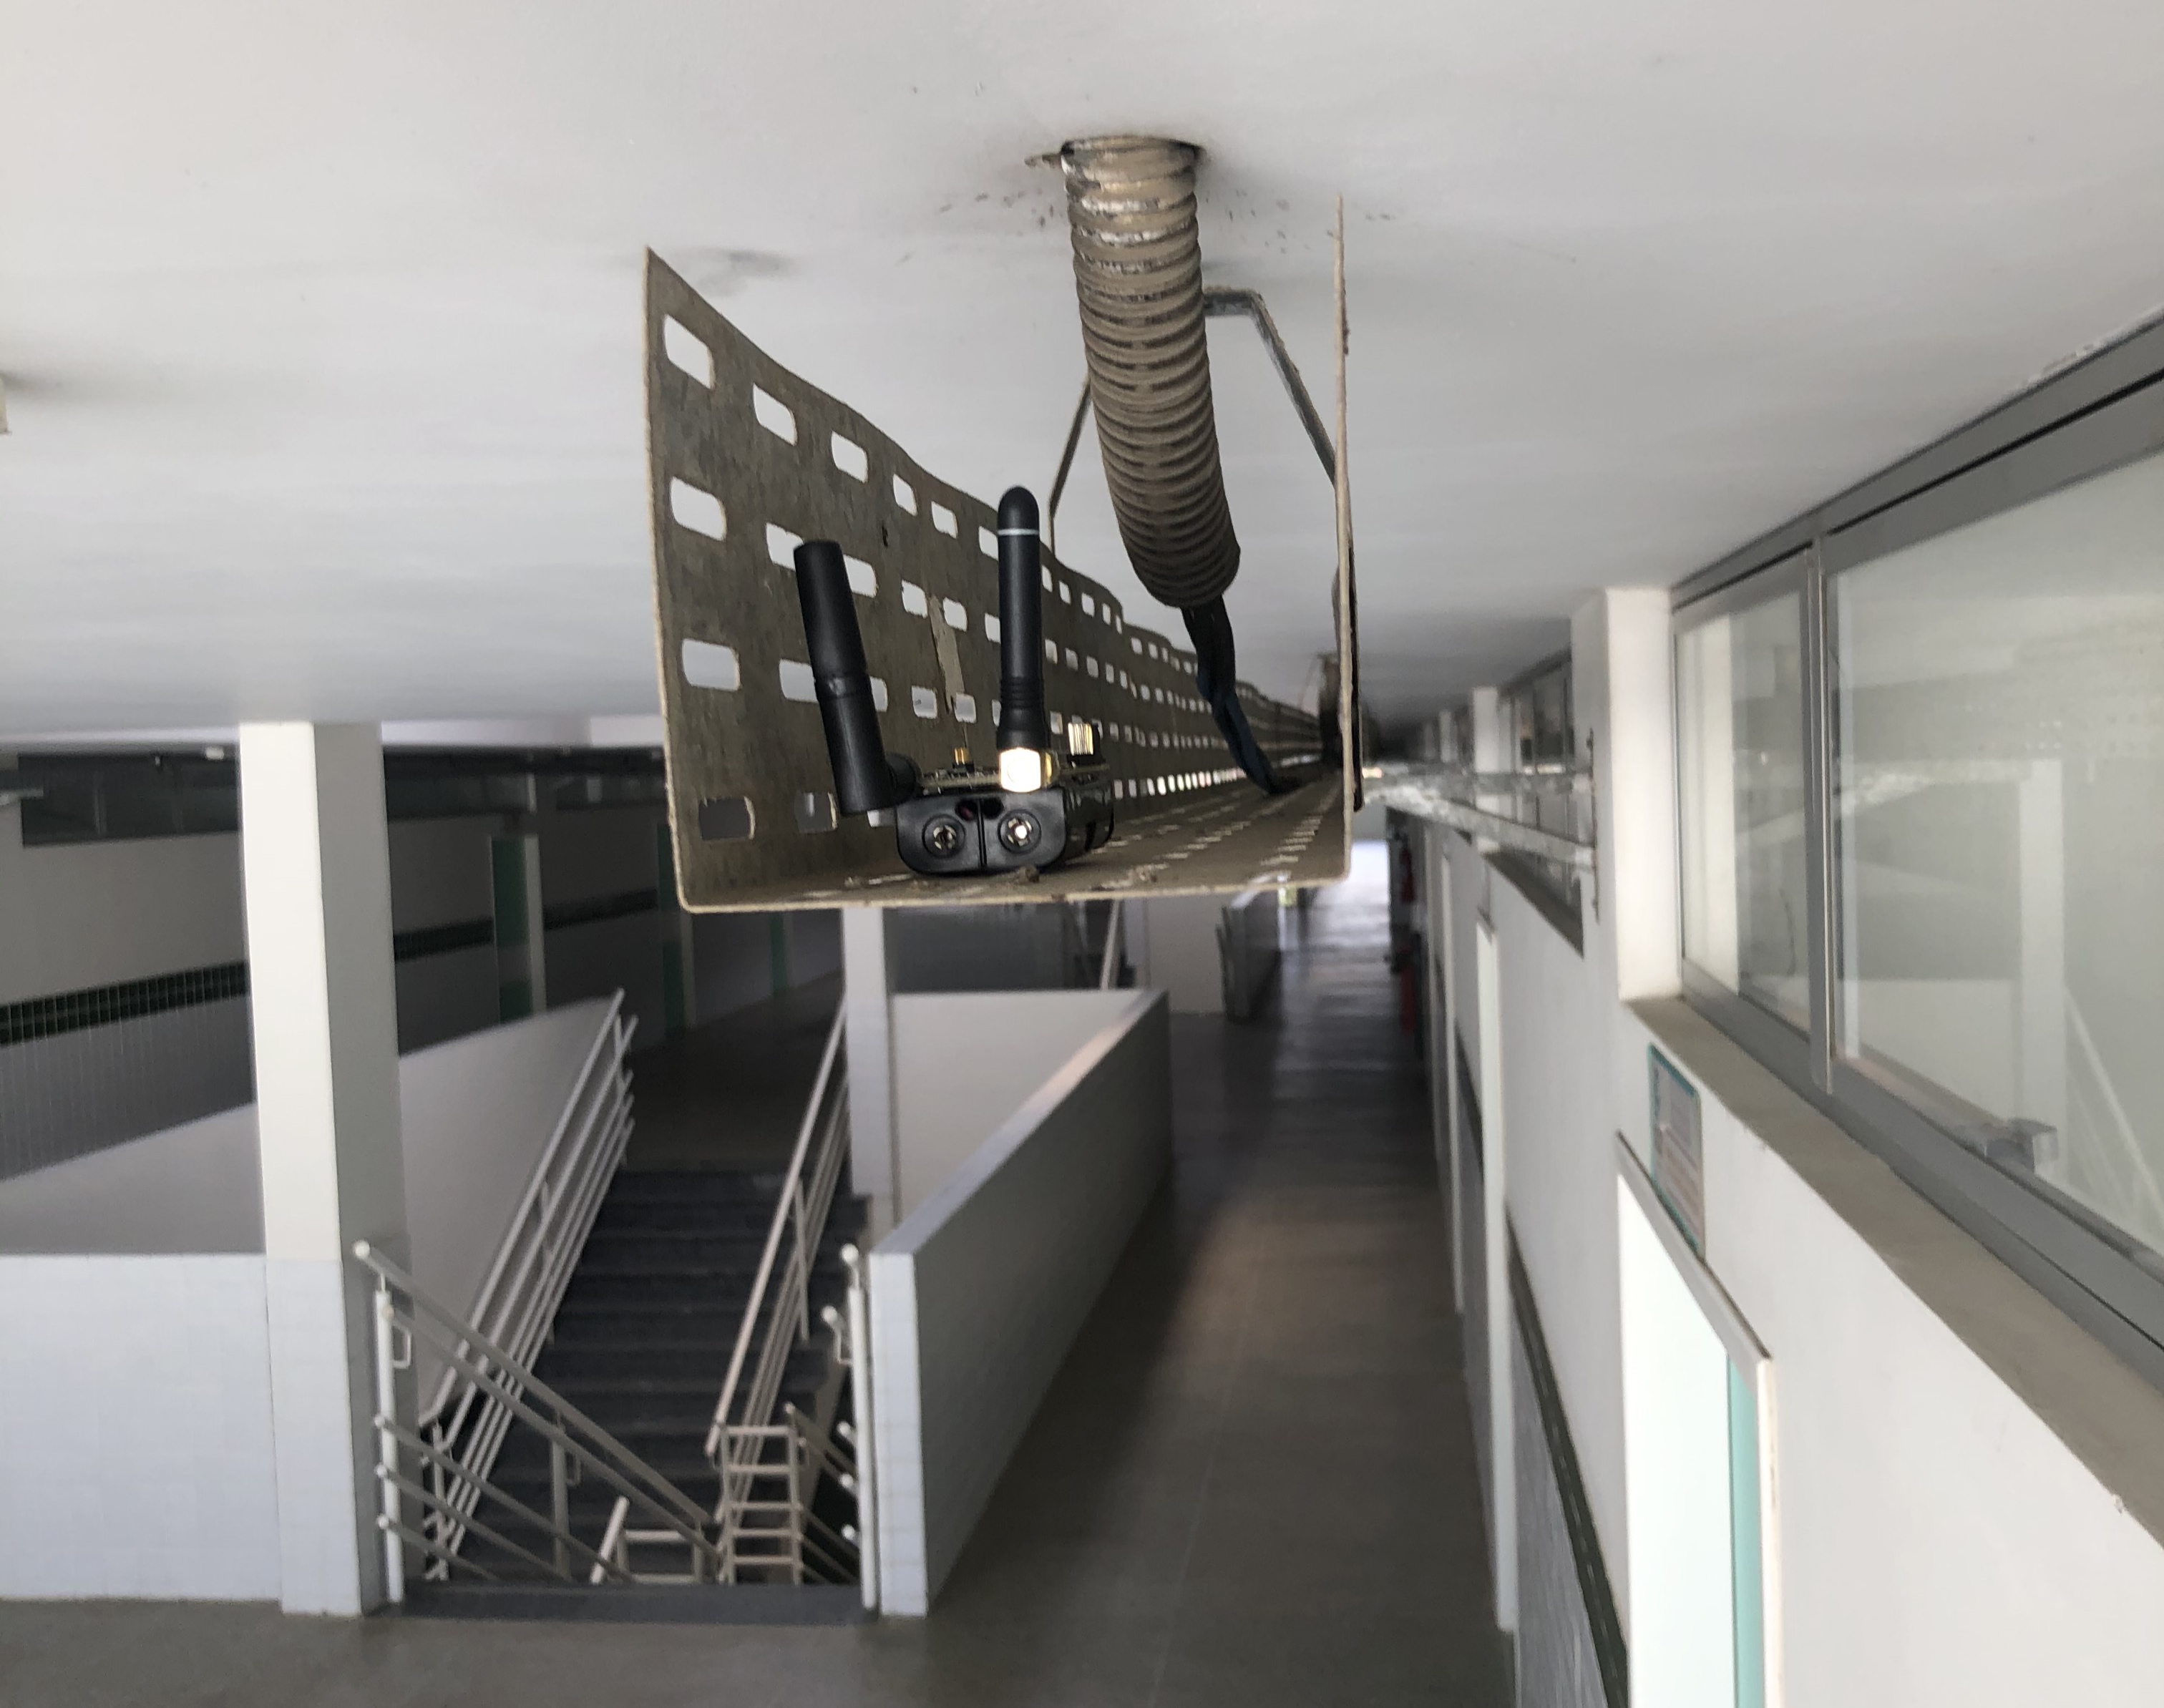
\includegraphics[width=0.7\textwidth]{resources/tx_canaleta.jpg}\\
      \footnotesize{Fonte autoral}
    \end{figure}
  \end{frame}

  \begin{frame}{Experimento}
    \framesubtitle{Visão Geral}
    \begin{figure}
      \centering
      \includegraphics[width=\textwidth]{resources/rede_visão_geral.png}\\
      \footnotesize{Fonte autoral}
    \end{figure}
  \end{frame}

  \begin{frame}{Experimento}
    \framesubtitle{OpenMote B}
    \begin{figure}
      \centering
      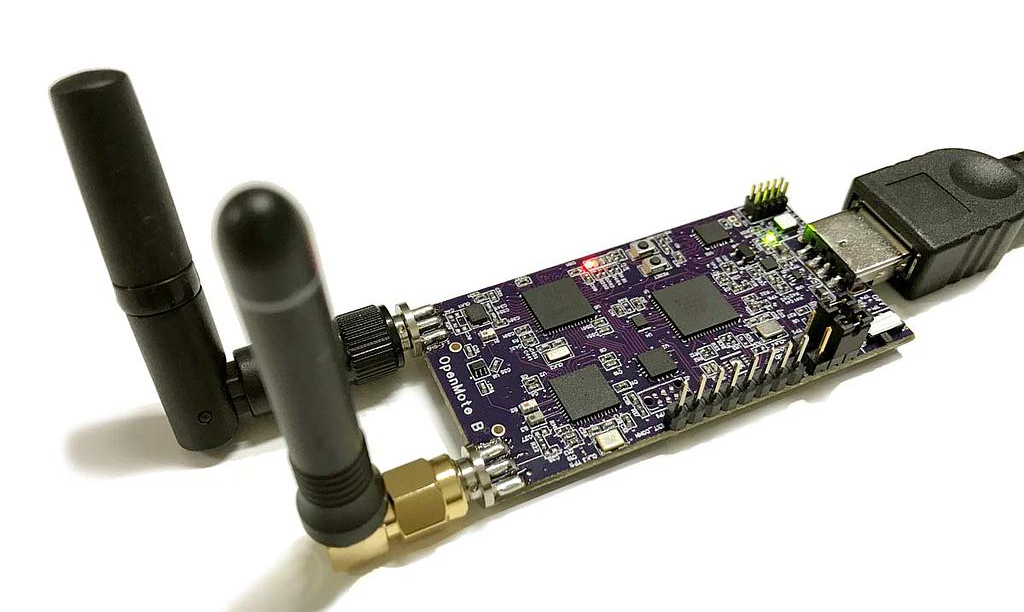
\includegraphics[width=.8\textwidth]{resources/openmote-b.jpg}\\
      \footnotesize{Fonte autoral}
    \end{figure}
  \end{frame}

  \begin{frame}{Experimento}
    \framesubtitle{Conteúdo das Mensagens}
    \begin{itemize}
      \item \alert{device\_id} \\ identificador dispositivo
      \item \alert{packet\_counter} \\ identificador auto incremental da mensagem transmitida
      \item \alert{tx\_mode} \\ número indicador da modulação utilizada na transmissão
      \item \alert{tx\_counter} \\ número indicador do ciclo de transmissão
    \end{itemize}
  \end{frame}
  \begin{frame}{Experimento}
    \framesubtitle{Conteúdo das Mensagens}
    \begin{itemize}
      \item \alert{csma\_retries} \\ número indicador da quantidade de tentativas da transmissão
      \item \alert{csma\_rssi} \\ número indicador da energia presente no canal de transmissão quando há uma tentativa de realizar a transmissão da mensagem
    \end{itemize}
  \end{frame}

  \begin{frame}{Experimento}
    \framesubtitle{OpenMote B}
    \begin{figure}
      \centering
      \includegraphics[width=\textwidth]{resources/ciclos.png}\\
      \footnotesize{Fonte autoral}
    \end{figure}
  \end{frame}

  \begin{frame}{Experimento}
    \framesubtitle{Recepção e Persistência dos Dados}
    \begin{block}{Dispositivos Receptores}
      \begin{itemize}
        \item \alert{Recebem} a sequência de \emph{bytes} via rádio
        \item \alert{Verifica} o valor de RSSI
        \item \alert{Envia} a sequência de \emph{bytes} pela interface serial
      \end{itemize}
    \end{block}

    \begin{block}{Script Python}
      \begin{itemize}
        \item \alert{Recebe} a sequência de \emph{bytes} via serial
        \item \alert{Decodifica} e \alert{estrutura}
        \item \alert{Armazena} no banco de dados
      \end{itemize}
    \end{block}
  \end{frame}



  \begin{frame}
    \usebeamerfont{title}%
    \usebeamercolor[fg]{title}%
    \vskip 0.5cm
    \raggedright Obrigado!
    \vskip-.5\baselineskip
    \begin{pgfpicture}
      \pgfsetlinewidth{2pt}
      \pgfsetroundcap
      \pgfsetdash{{0pt}{4pt}}{0cm}

      \pgfpathmoveto{\pgfpoint{0mm}{0mm}}
      \pgfpathlineto{\pgfpoint{\textwidth}{0mm}}

      \pgfusepath{stroke}
    \end{pgfpicture}

    % Input the subtitle
    \usebeamerfont{subtitle}%
    \usebeamercolor[fg]{subtitle}%
    \begin{minipage}{\textwidth}
      \raggedright%
      Felipe Ferreira Bezerra da Silva%
    \end{minipage}\vskip.25\baselineskip

    % Input the author's name
    \usebeamerfont{author}%
    \usebeamercolor[fg]{author}%

    \raggedright%
    felipeffbs3x@gmail.com
    \vskip 1cm

    \begin{figure}[b]
      
\includegraphics[width=.25\textwidth]{./fibeamer/logo/zut/ifpb.png}
      \hspace{1cm}
      
\includegraphics[width=.25\textwidth]{./fibeamer/logo/zut/gcompi.png}
    \end{figure}
  \end{frame}


\end{darkframes}
\end{document}
